Statistical inference lets us do 2 things:
\begin{enumerate}
	\item Estimating teh parameters of a statistical model
	\item Testing statistical hypotheses
\end{enumerate}
\section{Frequentist's point of view}
\subsection{Introduction}
This approach avoid treating parameters like random variables, and which thus avoid the 
use of priors and Bayes rule.


\subsection{Sampling distribution of an estimator}
In frequentist statistic a parameter estimate $\hat{\theta}$ is computed by applying an
estimator $\delta$ to some data $\mathcal{D}$, so $\hat{\theta}=\delta(\mathcal{D})$.
The uncertainty in the parameter estimate can be measured by computing the \emph{sampling
distribution} of the estimator.
Imagine sampling many different datasets $\mathcal{D}^{(s)}$ from some true model 
$p(\cdot|\theta^{*})$ meaning $\mathcal{D}^{(s)}=\left\{x_{i}^{(s)}\hookrightarrow 
p(\cdot|\theta^{*})\right\}_{1\leq i\leq N}$ for $1\leq s\leq S$ and $\theta^{*}$ is the 
true parameter. Now apply the estimator $\hat{\theta}(\cdot)$ to each $\mathcal{D}^{(s)}$
to get a set of estimates $\{\hat{\theta}(\mathcal{D}^{(s)})\}_{1\leq s\leq S}$.\\
As we late $S \rightarrow \infty$, the distribution induced on $\hat{\theta}(\cdot)$ is 
the \textbf{sampling distribution of the estimator}.

\paragraph{Bootstrap}
It is a simple \emph{Monte Carlo} technique to approximate the sampling 
distribution.
The idea is that if we knew the true parameters $\theta^{*}$, we could generate $S$ fake 
datasets of size $N$, from the true distribution. We could then compute our estimator from
each sample, and use the empirical distribution of the resulting samples as our estimate
of the sampling distribution.\\
Since $\theta$ is unknown, the idea of the \textbf{parametric bootstrap} is to generate
the samples using $\hat{\theta}(\mathcal{D})$ instead.
An alternative, called \textbf{non-parametric bootstrap} is to sample the $x_{i}^{s}$
(with replacement) from the original data $\mathcal{D}$ and then compute the induced
distribution as before.

\subsection{Fequentist decision theory}
In Frequentist decision theory there is a loss function and a likelihood, but there
is no prior and hence no posterior or posterior expected loss. Thus there is no 
automatic way of deriving an optimal estimator, unlike the Bayesian case.\\
Instead, we are free to choose any estimator or decision procedure $\delta: \mathcal{X}
\rightarrow \mathcal{A}$ we want.\\
Having chosen an estimator, we define its expected loss or risk as follows
\begin{center}
 $R(\theta^{*}, \delta) \triangleq \mathbb{E}_{p(\tilde{\mathcal{D}}|\theta^{*})}
\left(L(\theta^{*}, \delta(\tilde{\mathcal{D}}))\right) = \Su{}{}L\left(\theta^{*},
\delta(\tilde{\mathcal{D}})p(\tilde{\mathcal{D}})\right)d\tilde{\mathcal{D}}$   
\end{center}
where $\tilde{\mathcal{D}}$ is data sampled from 'nature's distribution' which is 
represented by parameter $\theta^{*}$.
Whereas the Bayesian posterior expected loss: 
\begin{center}
    $p(a, \mathcal{D, \pi}) \triangleq \mathbb{E}_{p(\theta|\mathcal{D},\pi)}\left(
        L(\theta, a) = \Su{\Theta}{}L(\theta, \bm{a})p(\theta|\mathcal{D}, \pi)d\theta
    \right)$
\end{center}
We see that the Bayesian approach averages over $\theta$, which is unknown, and conditions
on $\mathcal{D}$ which is known. Unlike the frequentist approach averages over $\tilde{
\mathcal{D}}$, thus ignoring the observed data, and conditions on $\theta^{*}$ which is 
unknown.

\paragraph{Bayes risk}
How to chose amongst the estimators? 
We need some way to convert $R(\theta^{*}, \delta)$ into single measure of quality, $R(
\delta)$ which does not depend on knowing $\theta^{*}$. One approach is to put a prior on
$\theta^{*}$ and then to define \textbf{Bayes risk} of an estimator as follows:
\begin{center}
    $R_{B}(\delta) \triangleq \mathbb{E}_{p(\theta^{*})}\left(R(\theta^{*}, \delta)\right)
    \Su{}{}R(\theta^{*}, \delta)p(\theta^{*})d\theta^{*}$
\end{center}
A \textbf{Bayes estimator} or \textbf{Bayes decision rule} is one which minimizes the 
expected risk: $\delta_{B} \triangleq \displaystyle\argmin_{\delta} R_{B}(\delta)$
\subparagraph{Connection Bayesian and Frequentist approaches to decision theory.}
\begin{itemize}
    \item \emph{Theorem 1} A Bayes estimator can be optained by minimizing the posterior 
        expected loss for each $\bm{x}$
    \item \emph{Theorem 2} Every admissible decision rule is a Bayes decision rule with 
        respect to some possibly improper prior distribution.
\end{itemize}
\subparagraph{Minimax risk}
Some frequentist statistic users avoid using Bayes risk since it requires the choice of
a prior, although this is only in the evaluation of the estimator, not necessarily as 
part of its construction. An alternative approach is as follows:
\begin{enumerate}
    \item Define the  maximum risk of an estimator as:\\
        $R_{max}(\delta) \triangleq \displaystyle\theta^{*}R(\bm{\theta}^{*},\delta)$
    \item A \textbf{minimax rule} is one which minimizes the maximum risk:
        $\delta_{MM} \triangleq \displaystyle\argmin_{\delta} R_{\max}(\delta)$
\end{enumerate}
Minimax estimators have a certain appeal, however computing them can be hard and 
furthermore they are very pessimistic.
In most statistical situations, excluding games theoretic ones, assuming nature is an
adversary is not a reasonable assumption.
\subparagraph{Admissible estimators}
The basic problem with frequentis decision theory is that it relies on knowing the true
distribution $p(\cdot|\theta^{*})$ in order to evaluate the risk. However it might be 
the case that some estimators are worse than others regardless of the value of 
$\theta^{*}$.\\
In particular if for $\theta \in \Theta, R(\theta, \delta_{1}) \leq R(\theta, \delta_{2})$
then we say that $\delta_{1}$ \textbf{dominates} $\delta_{2}$.\\
An estimator is said to be \textbf{admissible} if it is not strictly dominated by any 
other estimator.\\
\textbf{Admissibility is not enough}


\subsection{Desirable properties of estimators}
\subparagraph{Consistent estimators}
An estimator is said to be \textbf{consistent} if it eventually recovers the true
parameters that generated the data as the sample size goes to infinity. 

\subparagraph{Unbiased estimator}
The \textbf{bias} of an estimator is defined as 
\begin{center}
    $bias\left(\hat{\theta}(\cdot)\right) = \mathbb{E}_{p(\mathcal{D}|\theta^{*})}
    \left(\hat{\theta}(\mathcal{D})-\theta^{*}\right)$
\end{center}
The estimator is unbiased when the bias is equal to 0.

\subparagraph{Minimum variance estimators}
A famous result called the \textbf{Cramerè-Rao lower bound} provides a lower bound on the
variance of any unbiased estimator. More precisely:
Let $\left(X_{j}\right)_{1 \leq j \leq p} \hookrightarrow p(X|\theta_{0})$ and 
$\hat{\theta}(\cdot)$ an unbiased estimator of $\theta^{*}$
Then, under various smoothness assumptions on $p(X|\theta_{0})$ we have  
\begin{center}
    $\mathbb{V}(\hat{\theta}) \geq \dfrac{1}{nI(\theta^{*})}$
\end{center}
where $I(\theta^{*})$ is the Fisher information matrix.

\subparagraph{Bias-Variance Trade-off} 
As $MSE = variance + bias^{2}$\\
It might be wise to use a biased estimator, so long as it reduces our variance, assuming
our goal is to minimize squared error. 


\subsection{Empirical risk minimization}
Frequentist decision theory suffers from the fundamental problem that one cannot actually
compute the risk function, since it relies on knowing the true data distribution. By
contrast, the Bayesian posterior expected loss can always be computed since it conditions
on the data rather that on $\theta^{*}$.\\
However there is one setting which avoids this problem, it is when the task is to predict
observable quantities, as opposed to estimating hidden variables or parameters.\\
Instead of looking at loss functions of the form $L(\bm{\theta^{*}}, \delta(\mathcal{D}))$
let us look at loss functions of the form $L(y, \delta(\bm{x}))$.\\
Then the risk becomes:
$R(p_{*}, \delta) \triangleq \mathbb{E}_{(\bm{x}, y)\hookrightarrow p_{*}}\left(L(y,
\delta(\bm{x}))\right) = \su{\bm{x}}{}\su{\bm{y}}{}L(y, \delta(\bm{x}))p_{*}(\bm{x}, y)$
Where $p_{*}$ represents "nature's distribution", indeed this distribution is unknown, 
but a simple approach is to use the empirical distribution, derived from some training 
data to approximate $p_{*}$
$p_{emp} \triangleq \dfrac{1}{N}\su{i=1}{N}\delta_{x_{i}}(\bm{x})\delta_{y_{i}}(y) 
\approx p_{*}(\bm{x}, y)$
We define the empirical risk as follows:
\begin{center}
    $R_{emp}(\mathcal{D}, \mathcal{D}) \triangleq R(p_{emp}, \delta) = \dfrac{1}{N}
    \su{i=1}{N}L(y_{i}, \delta(x_{i}))$
\end{center}
\subparagraph{Regularized risk minimization}
\begin{center}
    $R'(\mathcal{D}, \delta) = R_{emp}(\mathcal{D}, \delta) + \lambda C(\delta)$
\end{center}
where $C(\delta)$ measures the complexity of the prediction function $\delta(\bm{x})$ and 
$\lambda$ controls the strength of the complexity penalty. 
This approach is known as \textbf{regularized risk minimization}.

\paragraph{Estimating the risk using cross validation}
Principle of cross validation













\subsection{Tools}
\paragraph{Introduction}
Avoid treating parameters as randome variables.
The notion of variation across repeated trials forms the basis for modelling
uncertainity.


\paragraph{Hypothesis Testing}
A \emph{frequentist} statistics, probabilities represent the frequencies at which 
particular events happen.

\paragraph{\emph{p-value}}
It is the heart of frequentist hypothesis testing, it tells us the probability of getting
a particular test statistic $t$ as big as the one we have or bigger under the null 
hypothesis (that there is actually no effect).\\
By convention we usually conclude an effect is \emph{statistically significant} if the 
\emph{p-value} is less than a threshold $\alpha$.

\paragraph{Confidence intervals}
When we fit a model to our data we look for the \emph{maximum of likelihood} parameters,
meaning the parameters that are most consistent with our data. 
For each parameter we will able to construct $95\%$ interval namely $95$ of the $100$ 
intervals generated will contain the true value of the parameter.\\
If $H_{0}: \beta=0$ is true, the probability of getting a $95\%$ confidence interval that
does not include 0 is less than 0.05. In other words, if the $95\%$ confidence does not 
include 0, $p<0.05$.
\begin{figure}[H]
	\begin{center}
		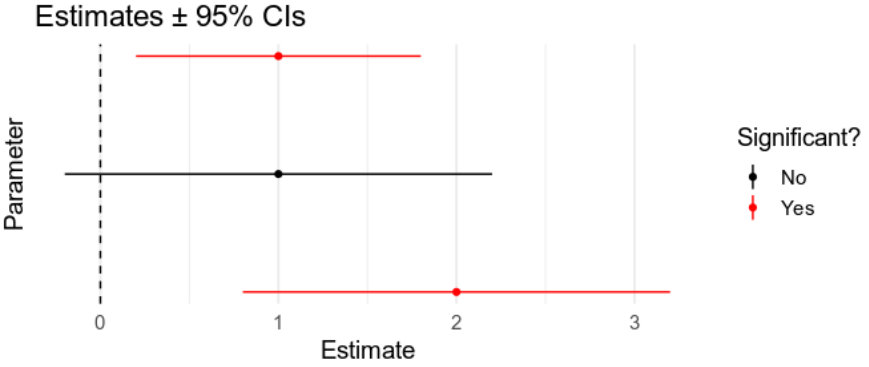
\includegraphics[width=\textwidth]{./chaps/10sec/images/4_estimates.png}
	\end{center}
	\caption{Confidence interval}
	\label{fig:4_estimates}
\end{figure}

\paragraph{Multiple comparisons}
The more tests we run the more likely it is to we'll find at least one that is significant
even though the null hypothesis is true. We can then apply a Bonferroni correction.\\
Let's say we are running $k$ tests, we can either adjust: 
\begin{itemize}
	\item the threshold $\alpha_{adj} = \dfrac{\alpha}{k}$ OR
	\item the \emph{p-value} $p_{ajd} = k\times p$
\end{itemize}


\section{Bayesian's point of view}
\subsection{Tools}

\paragraph{Summarizing posterior distributions}
\subparagraph{MAP}
Although most appropriate choice for:
$
\begin{cases}
	\text{Real valued quantity} &\rightarrow \text{\emph{posterior median or mean}}\\
	\text{Discrete} &\rightarrow \text{\emph{vector of posterior marginals}}
\end{cases}
$\\
The most popular choice is \tB{\emph{posterior mode}} aka \tR{MAP}, because it reduces to
optimization problems for which efficient algorithms often exist.\\
Some point to be aware about MAP:
\begin{itemize}
	\item \sB{No measure of uncertainty}
	\item \tB{Plugging in the MAP estimate can result in overfitting}
	\item \tB{The mode is an untypical point}, unlike the mean or median the mode is a
		point of measure 0, it does not take the volume of the space into account.
	\item \tB{MAP estimation is not invariant to reparameterization}, for example 
		passing from centimeters to inches can break things.)\\ The MLE does not
		suffer from this since the likelihood is a function not a probability
		density
\end{itemize}

\subparagraph{Credible Intervals}
With point estimates, we want a measure of confidence. 
\tB{
$$ C_{\alpha}\left(\mathcal{D}\right) = (l, u): \Prob{{l\leq \theta \leq u | \mathcal{D}}}
$$}
In general, credible intervals are usually what people want to compute but confidence
intervals are usually what they actually compute, because most people are taught 
frequentist statistics but not Bayesian statistics.\\
Sometimes with central intervals there might be points be outside the CI which have higher
probability density.\\
More formally $p^{*}$ such that: 
\begin{center}
	$1-\alpha = 
	\Su{{\theta:p(\theta|\mathcal{D})>p^{*}}}{}p(\theta|\mathcal{D})d\theta$
\end{center}
Then the \sB{HPD} such that:
\begin{center}
	$\mathcal{D}=\left\{\theta: p(\theta|\mathcal{D})\geq p^{*}\right\}$
\end{center}
\paragraph{Bayesian model selection}
A more efficient approach than cross-validation, meaning fitting \emph{k} times each
model, is to compute the posterior over models.
$$
p(m|\mathcal{D}) = \dfrac{p(\mathcal{D}|m)p(m)}{\su{{m\in\mathcal{M}}}{}p(m|\mathcal{D})}
$$
From this we can compute the \tB{MAP model $\hat{m} = \displaystyle \argmax_{m}
p(m|\mathcal{D})$}\\
Then we have the \tB{marginal likelihood}: $p(\mathcal{D}|\hat{m}) = \Su{}{}p(
\mathcal{D}|\hat{m})p(\theta|\hat{m})d\theta$
\subparagraph{Baysian Occam's razor}
In integrating out the parameters rather than maximizing them we are automatically 
protected from overfitting: model with more parameters do not necessarily have higher 
marginal likelihood.\\
A way to understand the Bayesian Occam's razor effect is to remember that probabilities 
must sum to one, meaning $\su{{\mathcal{D}'}}{}p(\mathcal{D}'|m)=1$. Complex models, which
can predict many things, must spread their probability mass thinly, and hence will not
obtain as large a probability for any given data set as simpler models.

\subparagraph{Computing the marginal likelihood (evidence)}
For a fixed model we often write:
$$p(\bm{\theta}|\mathcal{D},m) \propto p(\bm{\theta}|m)p(\mathcal{D}|\bm{\theta},m)$$
This valid since $p(\mathcal{D}|m)$ is constant. However when comparing models we need
to know how to compute the marginal likelihood, $p(\mathcal{D}|m)$. In general this can
be quite hard, since we have to integrate over all possible parameter values, but when
we have a conjugate prior, it is easy to compute.\\
Let $p(\bm{\theta})=\dfrac{q(\bm{\theta})}{Z_{0}}$ be our prior, where $q(\bm{\theta})$
is an unnormalized distribution, and $Z_{0}$ is the normalization constant of the prior.
Let $p(\mathcal{D}|\bm{\theta})=\dfrac{q(\mathcal{D}|\bm{\theta})}{Z_{l}}$ be the 
likelihood, where $Z_{l}$ contains any constant factors in the likelihood. Finally let
$p(\bm{\theta}|\mathcal{D})=\dfrac{q(\bm{\theta}|\mathcal{D})}{Z_{N}}$ be our posterior
where $q(\bm{\theta}|\mathcal{D})=q(\mathcal{D}|\bm{\theta})q(\bm{\theta})$ is the 
unnormalized posterior, and $Z_{N}$ is the normalization constant of the posterior.\\
We have:
$
\begin{cases}
	p(\bm{\theta})= \dfrac{p(\mathcal{D}|\bm{\theta})p(\bm{\theta})}{p(\mathcal{D})}\\
	\dfrac{q(\bm{\theta}|\mathcal{D})}{Z_{N}} = \dfrac{q(\mathcal{D}|\bm{\theta})
	q(\bm{\theta})}{Z_{l}Z_{0}p(\mathcal{D})}\\
	p(\mathcal{D}) = \dfrac{Z_{N}}{Z_{0}Z_{l}}
\end{cases}
$

In general $p(\mathcal{D}|m) = \Su{}{}p(\mathcal{D}|\bm{\theta})p(\bm{\theta}|m)d\bm{
\theta}$ can be quite difficult to compute. 
Simpler approach
\begin{itemize}
	\item \textbf{BIC} simple approximation:
		\tB{$BIC \triangleq \log(p(\mathcal{D}|\bm{\hat{\theta}})) - 
		\dfrac{dof(\bm{\hat{\theta})}}{2}\log(N)\approx\log{p(\mathcal{D})}$}
	\item \textbf{AIC}:
		\tB{$AIC(m,\mathcal{D})\triangleq\log(p(\mathcal{D})\bm{\hat{\theta}}_{MLE
		}) -dof(m)$}\\
		This is derived from Frequentits framework and cannot be interpreted as 
		an approximation to the marginal likelihood. The penalty of AIC is less
		than BIC, it causes AIC pick more complex models. That can be better for 
		predictive accuracy.
	\item Effect of the prior.\\
		If the prior is unknown, the correct Bayesian procedure is to put a prior
		on the prior. That is we should put a prior on the hyper-parameter 
		$\alpha$ as well as the parameters $\bm{w}$. To compute the marginal 
		likelihood we should integrate out all unknowns, we should compute:
		\tB{$\Su{}{}\Su{}{}p(\mathcal{D}|\bm{w})p(\bm{w}|\alpha,m)p(\alpha|m)
		d\bm{w}d\alpha$}
		A computational shortcut is to optimize $\alpha$ rather than integrating
		it out. That is, we use \tV{$p(\mathcal{D}|m)\approx\Su{}{}p(\mathcal{D}
		\bm{w})p(\bm{w}|\alpha,m)d\bm{w}$}.
		where \tV{$\hat{\alpha} = \displaystyle \argmax_{\alpha} p(\mathcal{D}|
			\alpha,m) = \displaystyle \argmax_{\alpha}\Su{}{}p(\mathcal{D}|
		\bm{w})p(\bm{w}|\hat{\alpha},m)d\bm{w}$}
\end{itemize}
\subparagraph{Bayes Factors}
When prior on models is uniform, then model selection is equivalent to picking the model
with the highest marginal likelihood. Now suppose we just have two models we are 
considering, call them the null hypothesis, $M_{0}$ and the alternative hypothesis,
$M_{1}$.\\
\tB{$$BF_{1,0} \triangleq \dfrac{p(\mathcal{D}|M_{1})}{p(\mathcal{D}|M_{0})}=
	\dfrac{\frac{p(M_{1}|\mathcal{D})}{p(M_{0}|\mathcal{D})}}{\frac{p(M_{1})}{
	p(M_{0})}}
$$}
This is like a likelihood ratio, except we integrate out the parameters, which allows us
to compare models of different complexity. 
\begin{table}
	\begin{tabular}{|cl|}
		\hline
	\textbf{Bayes Factor} $\bm{BF(1,0)}$ & \textbf{Interpretation}\\
		\hline
		$BF<\frac{1}{100}$ & Decisive evidence for $M_{0}$\\
		\hline
		$BF<\frac{1}{10}$ & Strong evidence for $M_{0}$\\
		\hline
		$\frac{1}{10}<BF<\frac{1}{3}$ & Modest evidence for $M_{0}$\\
		\hline
		$\frac{1}{3}<BF<1$ & Weak evidence for $M_{0}$\\
		\hline
		$1<BF<3$ & Weak evidence for $M_{1}$\\
		\hline
		$3<BF<10$ & Modest evidence for $M_{1}$\\
		\hline
		$BF>10 $ &  Strong evidence for $M_{1}$\\
		\hline
		$BF>100$ & Decisive evidence for $M_{1}$\\
		\hline
	\end{tabular}
\end{table}

\subparagraph{Jeffreys-Lindley paradox}
Problems can arise when we use improper priors (i.e. priors that do not integrate to 1)
for model selection/ hypothesis testing, even though such priors may be acceptable for 
other purposes. Thus it is important to use proper priors when doing model selection.

\paragraph{Priors}
The most controversial aspect of Bayesian statistics is its reliance on priors
\subparagraph{Uninformative priors}
If we do not have strong evidence on what $\theta$ should be, it is common to use an
uninformative priors, to "let the data speak for itself".\\
One might think that the most uninformative prior would be the uniform distribution: 
$Beta(1, 1)$, but the posterior would then be: $\E{\theta|\mathcal{D}} =
\dfrac{N_{1}+1}{N_{1}+N_{0}+2}$, whereas the MLE is $\dfrac{N_{1}}{N_{1}+N_{0}}$.\\
As by decreasing the magnitude of the pseudo counts, we can lessen the impact of the 
prior, we can argue that the most non-informative prior is: 
$$\lm{\epsilon}{0} Beta(\epsilon, \epsilon) = Beta(0, 0)$$
Called the \emph{Haldane prior}, it is an improper prior.\\
In general it is advisable to perform a some kind of sensitivity analysis, in which one
checks how much one's conclusions or prediction change in response to change in the 
modelling assumptions which includes the choice of the prior and the likelihood as well.
If the conclusion are relatively insensitive to the modelling assumption, one can have
more confidence in the results.
\subparagraph{Jeffreys priors}
Harold Jeffreys designed a general purpose technique for creating non-informative priors.
The key observation is that if $p(\phi)$ is non-informative then any re-parametrization
of the prior, such as $\theta=h(\phi)$ for some function $h$ should also be 
non-informative.
\begin{itemize}
	\item Start with a variable change: $p_{\theta}(\theta) = p_{\phi}(\phi)\left|\dfrac{d\phi}{d\theta}\right|$
	\item Consider the following constraint: $p_{\phi}(\phi)\propto
		\sqrt{\mathcal{I}(\phi)}$, where $\mathcal{I}(\phi)$ is the Fisher 
		information.\\ $\mathcal{I}(\phi) \triangleq - \E{2 \times 
		\dfrac{d\log\left(p(X|\phi)\right)}{d\phi}}$. This a measure of the
		curvature of the expected negative log likelihood and hence a measure of
		stability of the MLE.
	\item Now $\dfrac{d\log(p(x|\theta))}{d\theta} = 
		\dfrac{d\log(p(X|\phi))}{d\phi}\dfrac{d\phi}{d\theta}$
	\item $\mathcal{I}(\theta) = \mathcal{I}(\phi)
		\left(\dfrac{d\phi}{d\theta}\right)^{2}$
	\item $\sqrt{\mathcal{I}(\theta)} = \sqrt{\mathcal{I}(\phi)}\left|\dfrac{d\phi}
		{d\theta}\right|$
	\item Finally $p_{\theta}(\theta) = p_{\phi}(\phi)\left|\dfrac{d\phi}
		{d\theta}\right| \propto \sqrt{\mathcal{I}(\phi)}\left|\dfrac{d\phi}
		{d\theta}\right| = \sqrt{\mathcal{I}(\theta)}$
\end{itemize}

\subparagraph{Robust priors}
To prevent an undue influence on the result, we build priors having heavy tails, which 
avoids forcing things to be too close to the prior mean.

\subparagraph{Mixture of conjugate priors}
Conjugate priors simplify the computation of robust priors, but are often not robust, and 
not flexible enough to encode our prior knowledge. However it turns out that a mixture of
conjugate priors is also conjugate, and seem to be a good compromise.

\paragraph{Hierarchical Bayes}
A key requirement for computing the posterior $p(\theta|\mathcal{D})$ is the 
specification of a prior $p(\theta|\eta)$ where $\eta$ are the hyper-parameters. A 
Bayesian approach is to put a prior on our priors. This is an example of a \textbf{
hierarchical Bayesian Model}.

\paragraph{Empirical Bayes}
In hierarchical Bayesian models, we need to compute the posterior on multiple levels of
latent variables. For example, in a two-level model, we need to compute:
$p(\eta, \theta|\mathcal{D}) \propto p(\mathcal{D}|\theta)p(\theta|\eta)p(\eta)$\\
We can approximate the posterior on the hyper-parameters with a point-estimate, 
$p(\eta|\mathcal{D}\approx \delta_{\hat{\eta}}(\eta))$ where $\hat{\eta}=\argmax_{\eta}
p(\eta|\mathcal{D})$. Since $\eta$ is typically much smaller than $\theta$ in 
dimensionality, it is less prone to overfitting, so we can safely use a uniform prior on 
$\eta$. Then the estimate becomes: 
$$ \hat{\eta} = \argmax_{\eta} p(\mathcal{D}|\eta) = \argmax_{\eta} \Su{}{}
p(\mathcal{D}|\theta)p(\theta|\mathcal{\eta})d\theta $$
This overall approach is called \textbf{Empirical Bayes}\\
Empirical Bayes violates the principle that the prior should be chosen independently of 
the data. However, we can just view it as a computationally cheap approximation to 
inference in a hierarchical Bayesian model, just as we viewed MAP estimation as an approximation to inference in the one level model $\theta \rightarrow \mathcal{D}$. In fact, we
can construct a hierarchy in which the more integrals one performs, the "more Bayesian" 
one becomes:
\begin{center}
	\begin{tabular}{|*{2}{l|}}
		\hline
		\textbf{Method} & \textbf{Definition} \\
		\hline
		Maximum likelihood & $\hat{\theta} = \argmax_{\theta} 
		p(\mathcal{D}|\theta)$ \\
		\hline
		MAP estimation & $\hat{\theta} = \argmax_{\theta} 
		p(\mathcal{D}|\theta)p(\theta|\eta)$ \\
		ML-II (Empirical Bayes) & $\hat{\eta}=\argmax_{\eta}\Su{}{}
		p(\mathcal{D}|\theta)p(\theta|\eta)d\theta = \argmax_{\eta}p(\mathcal{D}|
		\eta)$ \\
		\hline
		MAP-II & $\hat{\eta}=\argmax_{\eta}\Su{}{}
		p(\mathcal{D}|\theta)p(\theta|\eta)p(\eta)d\theta = \argmax_{\eta}p(
		\mathcal{D}| \eta)p(\eta)$\\
		\hline
		Full Bayes & $p(\theta, \eta|\mathcal{D}) \approx p(\mathcal{D}|\theta)
		p(\theta|\eta)p(\eta)$\\
		\hline
	\end{tabular}
\end{center}

\paragraph{Bayesian decision theory}
We can formalize any given statistical decision problem as a game against nature (as 
opposed to a game against other strategic players, which is the topic of game theory).
In this game, nature picks a state or parameter or label, $y\in \mathcal{Y}$, unknown to 
us, and then generates an observation, $\bm{x}\in\mathcal{X}$ which we get to see. We then
have to make a decision, that is, we have to choose an action $a$ from some \textbf{action
space} $\mathcal{A}$.Finally we incur some \textbf{loss}, $L(y, a)$, which measures how
compatible our action $a$ is with nature's hidden state $y$.\\
Our goal is to devise a decision procedure or policy, $\delta: \mathcal{X}\rightarrow
\mathcal{A}$ which specifies the optimal action for each possible input which specifies the optimal action for each possible input, meaning the action that minimizes the expected 
loss:
$$ \delta(\bm{x}) = \argmin_{{a\in \mathcal{A}}} \E{{L(y, a)}}$$
In the Bayesian vision, the expected value of $y$ given the data we have seen so far, 
whereas in the frequentist vision the expected value refers to $x$ and $y$ that we expect
to see in the future.\\
In the Bayesian visionj the optimal action having observed $\bm{x}$ is defined as the 
action $a$ that minimizes the \textbf{posterior expected loss}:
$$ \rho(a|\bm{x})\triangleq\mathbb{E}_{p(y|x)}\left(L(y, a)\right) = \su{y}{}L(y, a)
p(y|x)$$
Hence the Bayes estimator also called Bayes decision rule is given by:
$$\delta(\bm{x}) = \argmax_{a\in\mathcal{A}}\rho(\bm{a}|\bm{x})$$

\subparagraph{Bayes estimators for common loss functions}
\begin{itemize}
	\item MAP estimate minimizes 0-1 loss: $L(y, a) = \mathbb{I}_{y\neq a}
		\begin{cases}
			0 \text{ if } a = y\\
			1 \text{ else}
		\end{cases}$
	\item Reject option, in classification problems where $p(y|\bm{x})$ is very 
		uncertain we may prefer to choose a reject action, in which we refuse to 
		classify the example as any of the specified classes. Let choosing $a=C+1$
		correspond to picking the reject action, and choosing $a\in\{1,...,C\}$
		correspond to picking one of the classes.\\
		$L(y=j, a=i) = 
		\begin{cases}
			0 &\text{ if } i=j \text{ and } i,j\in\{1,...,C\}\\
			\lambda_{r} &\text{ if } i=C+1 \\
			\lambda_{s} &\text{ otherwise}
		\end{cases} $\\
		where $\lambda_{r}$ is the cost of the reject action, and $\lambda_{s}$ is
		the cost of a substitution error. 
	\item Squared Error ($l_{2}$) for a continuous parameters. $L(y, a) = (y-a)^{2}$
	\item Absolute Error ($l_{1}$) more robust against outliers. $L(y,a)=
		\lvert y-a\rvert$. The optimal point is the median.

\end{itemize}



\paragraph{Hypothesis Testing}
A \emph{Bayesian} statistics, probabilities represent subjective beliefs. 
Bayesian hypothesis testing provides rules for calculating how you should update your 
beliefs about different hypotheses in light of the evidence you see.\\


\paragraph{Posterior belief}
We use distributions to represent model parameters, we are uncertain about.\\
We start out with \emph{prior distribution}, representing our belief before we have seen 
our data.\\
We then see some data, and the data will be more consistent with some parameters than 
others.\\
The rules of Bayesian inference tell us how to update our beliefs about the parameters now
that we've seen the data to obtain posterior beliefs.\\
Bayesian distributions are easy to interpret. The mode of the distribution is the most 
likely value of the parameter.
\begin{figure}[H]
	\begin{center}
		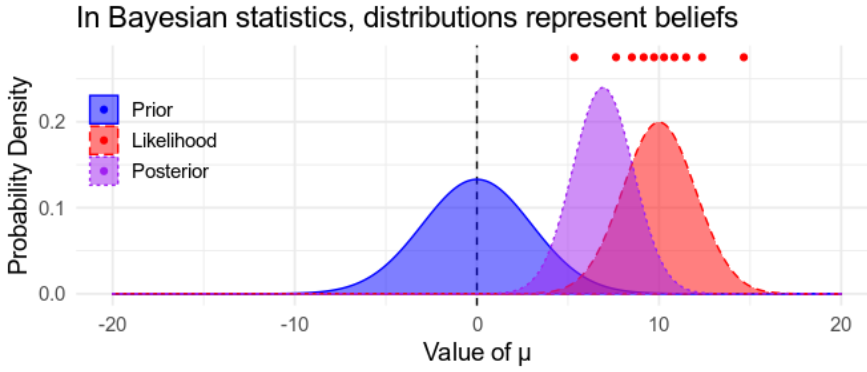
\includegraphics[width=\textwidth]{./chaps/10sec/images/2_posterior_belief.png}
	\end{center}
	\caption{Link between prior, likelihood and posterior}
	\label{fig:2_posterior_belief}
\end{figure}


\paragraph{Bayesian credible interval}
If $95\%$ of the distribution is between 2 values $\beta_{low}, \beta_{high}$ then 
according to the model there's a $95\%$ probability that the parameter is somewhere 
between these 2 values.\\
If we use uniform prior, the posterior distribution only depends on the data, and so we
end up with parameters that match the frequentist maximum-likelihood estimates: the 
posterior mode is the same as the maximum-likelihood value, and the credible intervals 
match the confidence intervals.
\begin{figure}[H]
	\begin{center}
		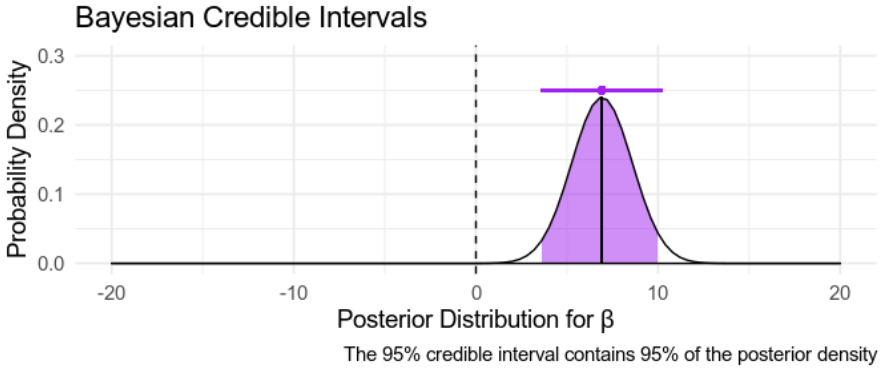
\includegraphics[width=\textwidth]{./chaps/10sec/images/1_credible_interval.png}
	\end{center}
	\caption{Bayesian Credible Intervals}
	\label{fig:1_credible_interval}
\end{figure}

\paragraph{Credible interval tests}
$95\%$ credible interval are commonly used as a simple way to decide whether an effect is
real or not: if the credible interval does not include 0, the effect is genuine. If it 
includes 0, it might not be.\\
If we use uniform prior, we can infer on the \emph{p-value}.

\paragraph{Posterior Sign tests}
Once we've calculated our posterior distribution for $\beta$, we can interrogate it 
directly. For instance if $99\%$ of the posterior distribution is above 0, we are $99\%$
sure that $\beta>0$ ($\prob{\beta>0}=0.99$) and $1\%$ sure that $\beta<0$.\\
However for example if our posterior distribution is centered on $0$ we find that 
$\prob{\beta>0}=\prob{\beta<0}=0.5$. The reason for this is that we are considering only
2 hypotheses, while ignoring that $\beta=0$. To test the hypothesis that $\beta=0$ we 
need to calculate the Bayes Factor.\\
Interestingly, the posterior sign test is closely 
\begin{figure}[H]
	\begin{center}
		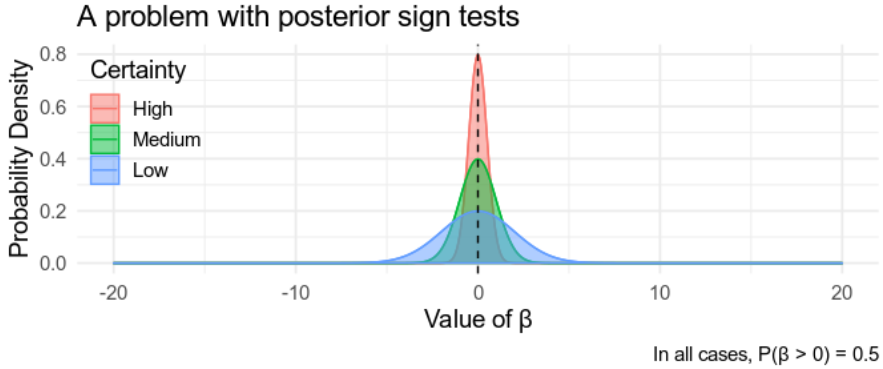
\includegraphics[width=\textwidth]{./chaps/10sec/images/3_sign_test.png}
	\end{center}
	\caption{Assessing certainty}
	\label{fig: 3_sign_test}
\end{figure}

\paragraph{Bayes Factors}
\subparagraph{Prerequisites}
$\probC{H_{0}}{Data}$ is a average over all possible values of $\beta$, weighted by how
likely each value in according to the prior.
$ \begin{cases}
	\probC{H_{1}}{Data} = \su{{i=1}}{n}\probC{\beta_{i}}{Data}\prob{\beta_{i}}\text{
		Discrete}\\
	\probC{H_{1}}{Data} = \Su{}{}\probC{\beta_{i}}{Data}\prob{\beta_{i}}\text{
		Continuous}
\end{cases} $
Setting an appropriate prior is complicated, usually initial parameters are left.

\subparagraph{Definition}
\begin{center}
	$BF_{10}=\dfrac{\probC{H_{1}}{Data}}{\probC{H_{0}}{Data}}$\\
	$BF_{01}=\dfrac{1}{BF_{10}}$\\
\end{center}
Note that in general it is easier to find evidence in favour $H_{0}$ if $H_{1}$ 
distribution is broad and easier to find evidence against $H_{0}$ if $H_{1}$ is narrow.
\begin{center}
	\begin{tabular}{|c|c|}
		\hline
		\textbf{Bayes Factor} & \textbf{Strength of evidence}\\
		\hline
		$BF=1$ & No evidence \\
		\hline
		$BF>1$ & Anecdotal evidence \\
		\hline
		$BF>3$ & Moderate \\
		\hline
		$BF>10$ & Strong \\
		\hline
		$BF>30$ & Very Strong \\
		\hline
		$BF>100$ & Extreme evidence \\
		\hline
	\end{tabular}
\end{center}

\subparagraph{Interpreting}
\textbf{Aim} : Finding how likely it is that $H_{1}$ is true and $H_{0}$ false.\\
Procedure: 
\begin{enumerate}
	\item Compute $BF_{10}$ using maximum-likelihood.
	\item Deciding how likely we thought it was the one or other hypothesis was true
		before seeing any data: \emph{the prior odds} $\prob{H_{1}}{H_{0}}$.\\
		Then there are 2 kinds of priors: prior beliefs about which hypothesis or 
		model is true, and prior beliefs about the values of the parameters in 
		each model.
	\item With the 2 above information compute the posterior distribution with Bayes'
		theorem\\ $\probC{Data}{H_{1}}=\dfrac{\probC{H_{1}}{Data}\prob{H_{1}}}{
		\probC{H_{0}}{Data}\prob{H_{0}}+\probC{H_{1}}{Data}\prob{H_{1}}}$
	\item 
\end{enumerate}
For example we get the following table:
\begin{center}
	\begin{tabular}{|*{4}{c|}}
		\hline
		$\mathbf{BF_{10}}$ & $\mathbf{BF_{01}}$ & \textbf{Prior} $\prob{H_{1}}$ &
		\textbf{Posterior} $\probC{Data}{H_{1}}$\\
		\hline
		$0.05$ & $20$ & $50\%$ & $4.8\%$\\
		\hline
		$0.1$ & $10$ & $50\%$ & $9.1\%$\\
		\hline
		$0.33$ & $3$ & $50\%$ & $25\%$\\
		\hline
		$1$ & $1$ & $50\%$ & $50\%$\\
		\hline
		$3$ & $0.33$ & $50\%$ & $75\%$\\
		\hline
		$10$ & $0.1$ & $50\%$ & $90.9\%$\\
		\hline
		$20$ & $0.05$ & $50\%$ & $95.2\%$\\
		\hline
	\end{tabular}
\end{center}


\paragraph{Multiple comparisons}
\subparagraph{Density Ratios}
\subparagraph{Posterior Estimates}
The more tests we run the more likely it is to we'll find at least one that is significant
even though the null hypothesis is true. We can then apply a Bonferroni correction.\\
Let's say we are running $k$ tests, we can either adjust: 
\begin{itemize}
	\item the threshold $\alpha_{adj} = \dfrac{\alpha}{k}$ OR
	\item the \emph{p-value} $p_{ajd} = k\times p$
\end{itemize}


